\section{Power Characterization}

We characterized the power consumption of drones when executing simple flight maneuvers as well as when executing macro-benchmarks person-tracking.

As a drone's size increases, its motors become responsible for a larger and larger portion of its power consumption, until the motors consume nearly all the power generated by a drone. Fig.~\ref{fig:power-hover-solo} illustrates the power distribution on a large MAV such as the 3DR Solo, while Fig.~\ref{fig:power-hover-nano} illustrates the power distribution of a much lighter and smaller nano-aerial vehicle such as the Hummingbird.

\begin{figure}[h]
\centering

  \subfloat[Large micro-aerial vehicle.]
  {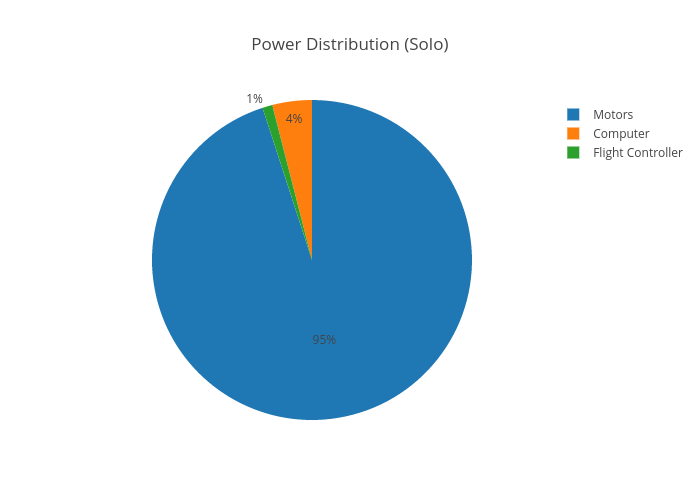
\includegraphics[width=.9\linewidth]{figs/power-hover-solo}
  \label{fig:power-hover-solo}}

  \subfloat[Small nano-aerial vehicle.]
  {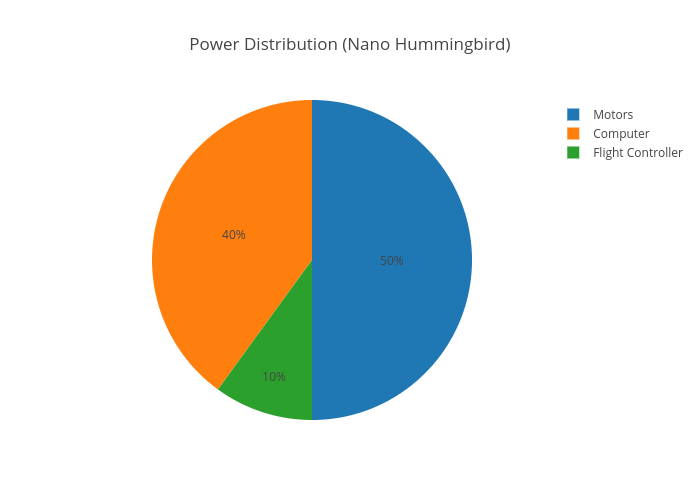
\includegraphics[width=.9\linewidth]{figs/power-hover-nano}
  \label{fig:power-hover-nano}}

\caption{Resolution vs performance on the drone.}
\label{fig:power-distribution}
\end{figure}

Thus, as a drone's size falls, it's flight time increasingly depends upon the power consumed by its companion computer, as well as the power required to lift its computer into the air. In Fig.~\ref{fig:flight-time-tracking-tx1}, we plot the flight time of our drones when executing the \textit{Person Tracking} benchmark. The drones are equipped with a TX1 giving them 20 FPS performance.

\begin{figure}[h]
\centering
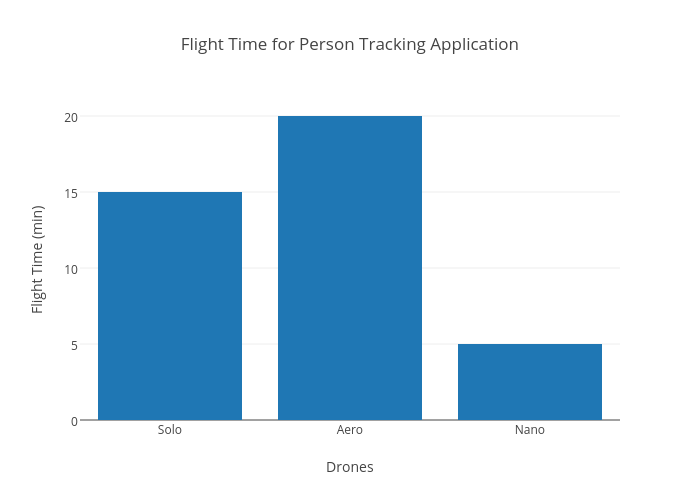
\includegraphics[width=\linewidth]{figs/flight-time-tracking-tx1}
\caption{Flight time of drones when executing \textit{Person Tracking} benchmark with TX1.}
\label{fig:flight-time-tracking-tx1}
\end{figure}

In Fig.~\ref{fig:perf-tracking-10min}, on the other hand, we plot the performance of the \textit{Person Tracking} application when running on various drones equipped with the most performant computer that will allow them to achieve 10 minutes of flight time.

\begin{figure}[h]
\centering
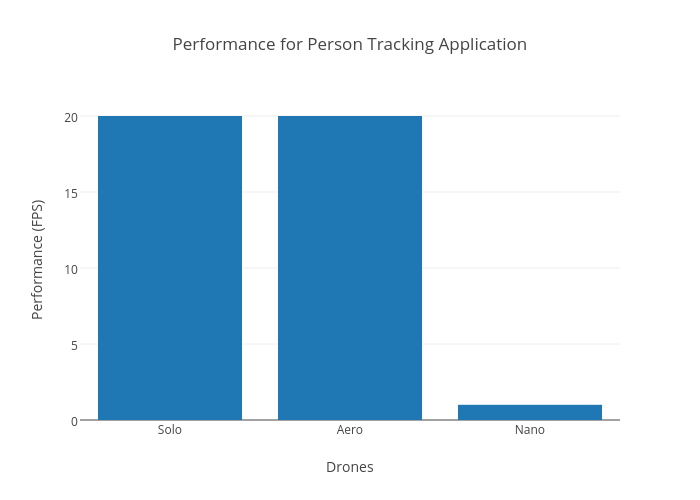
\includegraphics[width=\linewidth]{figs/perf-tracking-10min}
\caption{Performance of drones when executing \textit{Person Tracking} benchmark with 10 minutes of flight time.}
\label{fig:perf-tracking-10min}
\end{figure}

In Fig.~\ref{fig:energy-search-and-rescue}, we plot the total energy spent by our simulated AirSim drone when completing the \textit{Search-and-Rescue} macrobenchmark with various companion computers. As more powerful computers are used, our simulated drone is able to fly faster without missing potential targets and is thus able to complete its mission faster with less total energy expenditure.

\begin{figure}[h]
\centering
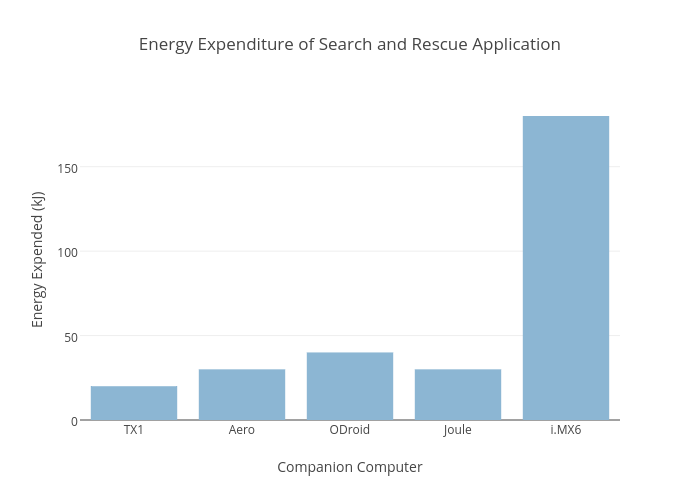
\includegraphics[width=\linewidth]{figs/energy-search-and-rescue}
\caption{Energy expended by AirSim drone when executing \textit{Person Tracking} benchmark with various companion computers.}
\label{fig:energy-search-and-rescue}
\end{figure}
